
\begin{frame}
  \frametitle{Sources of Error}
  \begin{figure}[h!]
    \centering
    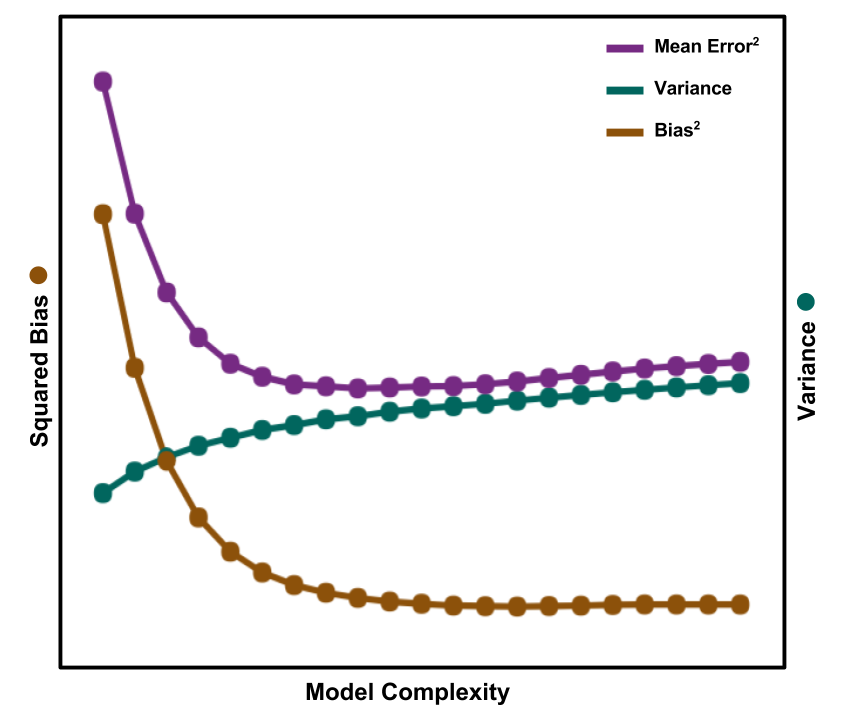
\includegraphics[height=0.7\textheight]{./figures/BVtradeoff.png}
    \caption{Bias and variance comprise the prediction error}
  \end{figure}
\end{frame}

\begin{frame}
  \frametitle{Types of Error}
  \begin{figure}[h!]
    \centering
    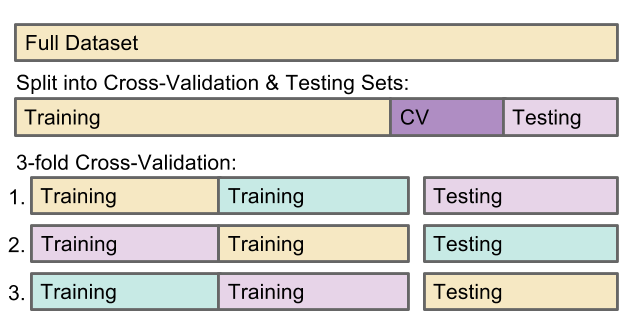
\includegraphics[width=0.8\textwidth]{./figures/cverror.png}
    \caption{Diagram explaining the concept of \textit{k}-fold cross-validation}
  \end{figure}
\end{frame}

\begin{frame}
  \frametitle{Error Metrics}
  L1, L2: absolute error and squared error
  
  Others: r2 score, percent error 

  Used for model prediction error and optimization of algs in obj funcs
\end{frame}
